%===================================
%===================================
%===================================
\setchapterpreamble[u]{\margintoc}
\chapter{Modelling overview}
\labch{intro:modelling}

%===================================
%===================================
\section{Performance metrics}
\labsec{intro:modelling:metrics}

To evaluate the quality of the models fit to the experimental data, four
performance metrics were evaluated: coefficient of determination (R$^2$),
\gls[format=long]{rmseLabel}, \gls[format=long]{maeLabel} and
\gls[format=long]{mapeLabel}. These metrics are described below.


\textbf{Coefficient of determination}. R$^2$ measures the proportion of the
variance in the predicted variable that can be attributed to the independent
variable(s), in this case the considered system inputs. Values close to one
indicate a better prediction accuracy. It is calculated as follows:

\begin{equation*}
    R^2 = 1 - \frac{\sum\limits_{i=1}^n (y_i - \hat{y}_i)^2}{\sum\limits_{i=1}^n (y_i - \bar{y})^2},
\end{equation*}

where $y_i$ is the measured or observed value for the output variable, in the
$i-th$ observation, $\hat{y}_i$ is the estimated value of the same variable and
$n$ is the total number of observations. Finally, $\bar{y}$ is the mean value
of the experimental values.


\textbf{Root Mean Square Error}. \gls{rmseLabel} is a statistical measure of
the difference between the values predicted by a model and the observed values.
It is calculated as the square root of the mean of the squared differences
between the predicted and observed values and it has its units. 

% \marginnote{
\begin{equation*}
    \mbox{RMSE} = \sqrt{\frac{1}{n} \sum\limits_{i=1}^n (y_i - \hat{y}_i)^2}
\end{equation*}
% }

\textbf{Mean Absolute Error}. It represents the average absolute difference
between predicted and actual values.

\begin{equation*}
    \mbox{MAE} = \frac{1}{n} \sum\limits_{i=1}^n \left|y_i - \hat{y}_i\right|
\end{equation*}

\textbf{Mean Absolute Percentage Error}. As the \gls{maeLabel}, it calculates
the difference between the predicted and the actual values, but in this case it
does so in relative terms:

\begin{equation*}
    \mbox{MAPE} = \frac{1}{n} \sum\limits_{i=1}^n \left| \frac{y_i - \hat{y}_i}{y_i} \right| \times 100\%
\end{equation*}



%===================================
%===================================
\section{First principle modelling}
\labsec{intro:modelling:first-principle}

%===================================
%===================================
\section{Data-driven modelling}
\labsec{intro:modelling:data-driven}

Machine learning algorithms are unique in their ability to obtain models and
extract patterns from data, without being explicitly programmed to do so. They
are more effective with large volumes of data but can also be applied to build
steady state regression models with less information of a process.

%================================
\subsection{Gaussian Process Regression}
\labsec{intro:modelling:gpr}

%================================
\subsection{Artificial Neural networks}
\labsec{intro:modelling:ann}

\glspl[format=long]{annLabel}, as the name suggests, have a behavior similar to
biological neurons. Their structure is formed by a succession of layers, each
one composed by nodes (or neurons) and they receive as input the output of the
previous layer. This process is subsequently repeated until the final layer
which has a number of neurons equal to the number of outputs.

There are important aspects to be considered in the \gls{annLabel} model
design, such as the model configuration, the network architecture and the
network topology. They are discussed below.

% Configuraciones de modelo
\textbf{Model configuration}. If the model has more than one output, several
configurations are available for the implementation of the model as shown in
\reffig{intro:modelling:ann-model-configuration}. The first one is a
\gls{mimoLabel} configuration, where a single network receives all the inputs
and directly produces all predicted outputs. The second one is a cascade
structure. This cascading approach involves training a network (\textit{network
A} in  \reffig{intro:modelling:ann-model-configuration} (b)) to predict one
output using the available inputs. Subsequently, these inputs, along with the
output from the first-output-predicting network, are fed into a second network
(\textit{network B} in \reffig{intro:modelling:ann-model-configuration} (b))
that is in charge of forecasting the second output. This procedure can be
repeated as many times as desired. A potential advantage of this configuration
is that it may reduce the experimental data requirements to obtain satisfactory
results. A third option is the combination of both configurations, where some
networks may predict several outputs, while others are fed some of these
outputs as subsequently use them as inputs. 

\begin{marginfigure}[-7cm]
    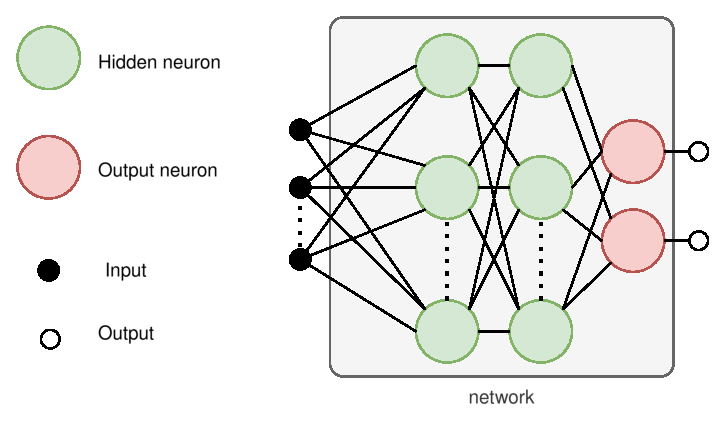
\includegraphics[]{figures/ann_model_configuration_mimo_with_legend.eps}
    {\footnotesize \textbf{(a)} \gls{mimoLabel} configuration\\}
    
    \vspace{1ex}
    
    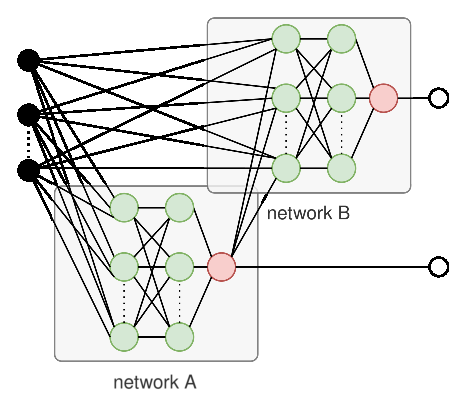
\includegraphics[]{figures/ann_model_configuration_cascade.eps}
    {\footnotesize \textbf{(b)} Cascade configuration}
    
    \caption{\acrshort{annLabel} model configurations}
    \labfig{intro:modelling:ann-model-configuration}
\end{marginfigure}

%As a result, this approach holds the promise of enhanced efficiency in model
%training, potentially requiring fewer data points for accurate predictions. 

% Tipos de red Feedforward Cascade-forward Radial-basis
\textbf{Network architectures}. Three network architectures have been
implemented and tested:
\begin{enumerate}
    \item \gls{ffLabel} network - \reffig{intro:modelling:ann-architectures}
    (a). This is the base network architecture, where different layers are
    added sequentially and the flow of information is unidirectional. The
    transfer function adopted in the hidden layers is the differentiable
    \textit{Log-Sigmoid}\sidenote{Defined as $logsig(x) = 1/(1 + e^{-x})$, mapping any real input to a value between 0 and
    1.}, whereas the one employed in the output layer is a linear one with no saturations.

    \item \gls{cfLabel} network - \reffig{intro:modelling:ann-architectures}
    (b). It is a variation on the feedforward network since it adds direct
    connections from the input and hidden layers to the output layer.

    \item \gls{rbfLabel} network - \reffig{intro:modelling:ann-architectures}
    (c). The transfer functions used in the first layer of the \gls{rbfLabel}
    network are different, they are local Gaussian like functions. Also,
    instead of multiplying by the weights, the distance between inputs and
    weights is computed and the bias is multiplied instead of added
    \sidecite{hagan_neural_2014}.
\end{enumerate}

% \begin{marginfigure}[]
%     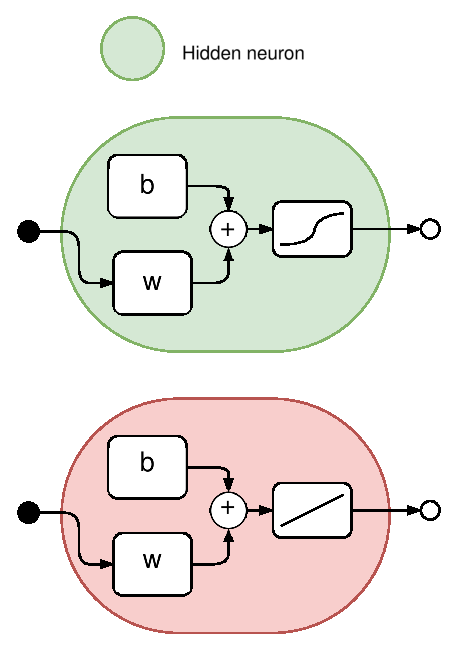
\includegraphics[]{figures/ann_neuron_type_simple_with_partial_legend.eps}
%     {\footnotesize \textbf{(a)} Feedforward\\} \vspace{2ex}
    
%     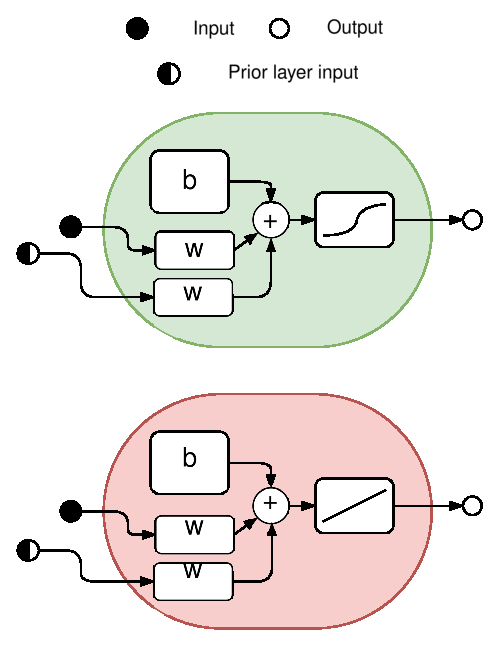
\includegraphics[]{figures/ann_neuron_type_cascade_with_partial_legend.eps}
%     {\footnotesize \textbf{(b)} Cascade-forward\\} \vspace{2ex}

%     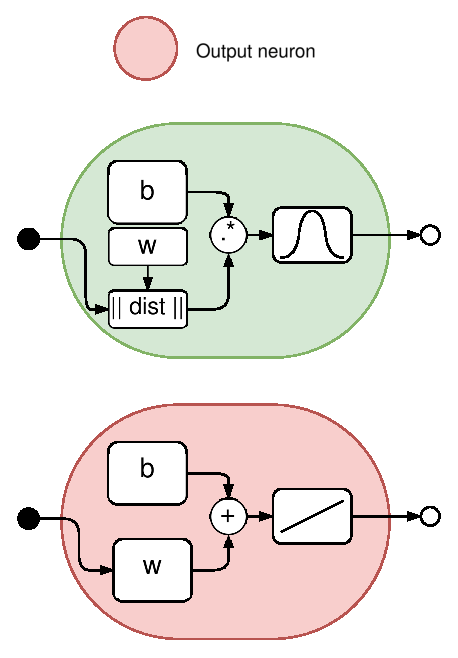
\includegraphics[]{figures/ann_neuron_type_radial_with_partial_legend.eps}
%     {\footnotesize \textbf{(c)} Radial-basis}

%     \caption{Considered \acrshort{annLabel} architectures}
%     \labfig{intro:modelling:ann-architectures}
% \end{marginfigure}

\begin{figure*}[h!]
    \centering
    \subfloat[\centering
    Feedforward]{{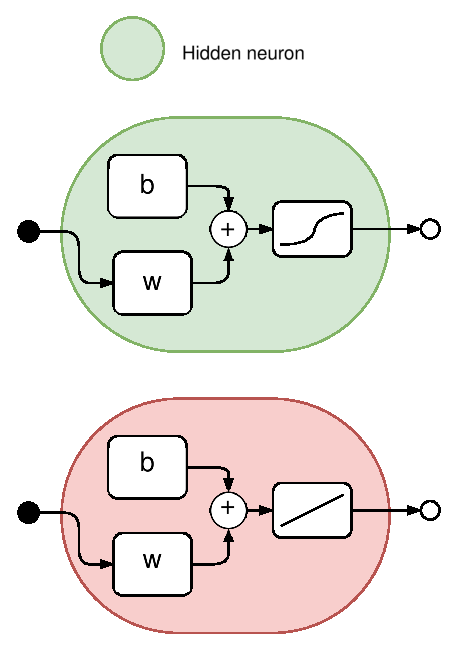
\includegraphics[width=0.32\textwidth]{figures/ann_neuron_type_simple_with_partial_legend.eps}
    }}%
    \qquad
    \subfloat[\centering
    Cascade-forward]{{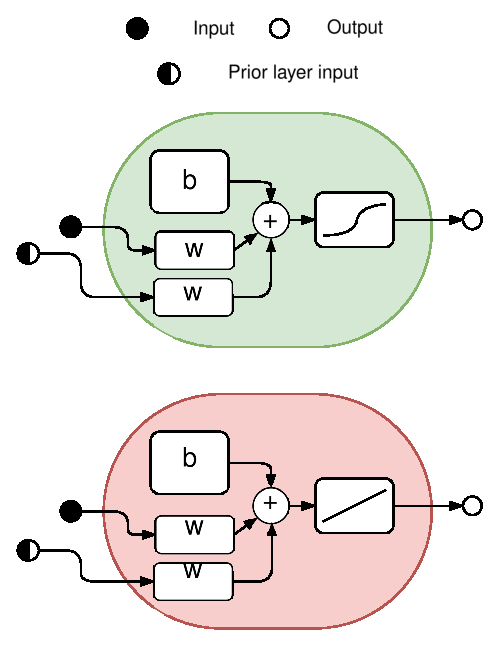
\includegraphics[width=0.32\textwidth]{figures/ann_neuron_type_cascade_with_partial_legend.eps}
    }}%
    \qquad
    \subfloat[\centering
    Radial-basis]{{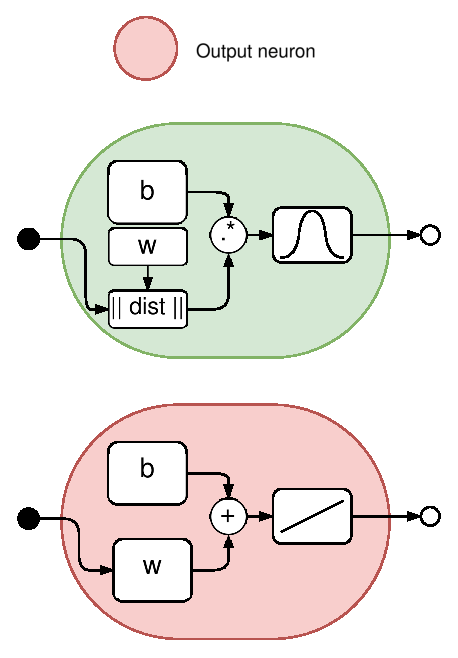
\includegraphics[width=0.32\textwidth]{figures/ann_neuron_type_radial_with_partial_legend.eps}
    }}%
    
    \caption{Considered \acrshort{annLabel} architectures}
    \labfig{intro:modelling:ann-architectures}
\end{figure*}

% topologías de red N de capas N de neuronas por capa

\textbf{Network topology}. Two-layer networks (one hidden and one output layer)
can learn almost any input-output relationship, including non-linear ones.
Adding more layers can improve the learning for more complex problems. However,
increasing the number of layers or neurons per layer increases the training
computational requirements, requires more data for a satisfactory model and can
lead to overfitting. Therefore, the process is usually started with two layers
and then the number of layers is increased if they do not perform
satisfactorily~\cite{hagan_neural_2014}. In this study, for the feedforward and
cascade-forward architectures, one and two hidden layers have been tested with
the following configurations: 5, 10, 20, 5-5, 5-10, 10-5, 10-10. For the case
of the \gls{rbfLabel}, it only has one hidden layer and neurons are added
sequentially during the training process up to a maximum which is set to 120
neurons.

% Procedimiento entrenamiento Justificar mejor elección de algoritmo de
% entrenamiento
\textbf{Training process}. The next important aspect to consider is the
training process. For the \gls{ffLabel} and \gls{cfLabel} networks many
Gradient- or Jacobian-based algorithms can be utilized. In this case, the
Levenberg-Marquardt backpropagation algorithm \sidecite{beale_neural_2010} has
been used. It is a fast algorithm, ideal for multilayer networks with up to a
few hundred weights and biases enabling efficient training. The training in
this case is done in batches since sequential training is slower and does not
produce better results. All data have been normalized applying the z-score
normalization method. 
% Early stop, paciencia For most applications of neural networks, the training
% error never converges to exactly zero. The error can reach zero for the
% perceptron network (radial basis network), but it is unlikely to happen for
% multilayer networks. For this reason, a criteria for deciding when to stop
% the training needs to be set in place, and this criteria needs provide a
% mechanism to avoid overfitting. 
The criteria established for deciding when to stop the training is the
following one:  when the performance on the validation set increases (worsens)
or when the  gradient is below a minimum ($1\times10^{-7}$) for a number of
iterations or epochs, or when a maximum number of 1000 epochs is reached. The
number of iterations to wait, often refereed as patience, is set to 6. Finally,
the selected network parameters will be those of the best epoch.

For each network architecture, the training process was repeated a total of ten
times (this is the recommended practice if the computational requirements allow
it, since it guarantees reaching a global optimum with a high degree of
confidence \sidecite{hamm_comparison_2007}). The optimal architecture and
training was selected according to a performance function, which in this case
has been the \gls{mseLabel} with the values normalized.

In the case of the \gls{rbfLabel} network, the chosen training method consists
in two stages which treats the two layers of the \gls{rbfLabel} network
separately. The first layer weights and biases are tuned based on the
orthogonal least squares method \sidecite{hagan_neural_2014}, while for the
second layer are computed in one step using a linear least-squares algorithm.
During training, neurons are added to the first layer (in increments of 20)
trying to minimize the \gls{mseLabel} to some goal, which in this case is set
depending on the case study: 10 for the \gls{mimoLabel} configuration and 0
($^\circ$C$^2$) and 20 (l$^2$/h$^2$) for temperature and water lost networks,
respectively, for the cascade configuration. Finally, a parameter called spread
is used to set the first layer biases. Larger values of this parameter promote
a smoother approximation of the training data (more generalization),
conversely, lower values provide a more exact fit to the training data. Values
from 0.1 to 30 have been tested for this parameter.


%================================
\subsection{Random Forest}
\labsec{intro:modelling::random-forest}

%================================
\subsection{Gradient Boosting}
\labsec{intro:modelling::gradient-boosting}

%===================================
%===================================
\section{Hybrid modelling}
\labsec{intro:modelling:hybrid}

%===================================
%===================================
\section[Data-driven from first-principles models. Sample generation]{Data-driven from first-principles models. Sample generation}[DD from FP. Sample generation]
\labsec{intro:modelling:sample-generation}

% Mencionar modelos basados en datos a partir de modelos físicos. Describir
% combinatoria sin detallar la combinatoria particular seguida para el modelo
% del CC.
One important advantage that first-principles models have over data-driven is
their scalability, that is, the ability to adapt a model developed and
validated in a pilot-scale system, to a large scale one. This is true for many
systems as long as the system configuration remains the same. This allows to
study and analyze pilot scale plants and extrapolate the results to industrial
sized plants. In addition, these type of model are also capable of predicting
the behaviour of the modelled systems in conditions that have not been tested
(\eg different operating or environmental conditions), although the
reliability of the model could be lower if these conditions move away from
those experimentally used for some parameter calibration.

On the contrary, data-driven models are very specific to the system and
operating ranges they are trained for. That is why training/calibrating a
data-driven model with data from a first-principles model is a common practice
to obtain a model that can be used in a larger range of operating conditions...

The process of generating samples from a first-principles model to train a
data-driven model is called sample generation. It consists of running the
first-principles model for a set of input parameters, which can be selected
randomly or following a specific distribution, and then using the outputs of
the first-principles model as the training data for the data-driven model.

The first step is to define the input parameters and their ranges. This can be
done by selecting the most relevant parameters for the system and determining
their ranges based on the system's operating conditions. The next step is to
generate a set of input parameters, which can be done using different methods
such as Latin Hypercube Sampling, Monte Carlo Sampling, Sobol Sampling, or
simply grid sampling. These methods allow to generate a set of input parameters
that cover the entire range of the input parameters and ensure that the
generated samples are representative of the system's behaviour. Once the input
parameters are defined, the first-principles model is run for each set of input
parameters, and the outputs of the model are recorded. Finally, the recorded
outputs are used to train the data-driven model.

\section{Hybrid modelling by means of \glspl{fsmLabel}}
\labsec{intro:modelling:fsm}

A state machine is a model of behavior composed of a finite number of
\textit{states} and \textit{transitions} between those states. Within each
state and transition some \textit{action} can be performed. A state machine
needs to start at some \textit{initial state}.

% TODO: Diagrama de FSM

Core concepts description:

\begin{itemize}
    \item \textbf{State}. A state represents a particular condition or stage in
    the state machine. It's a distinct mode of behavior or phase in a process.
    
    \item \textbf{Transition}. This is the process or event that causes the
    state machine to change from one state to another.

    \item \textbf{Action}. Specific operation or task that is performed when a
    certain event happens \ie a state is entered, exited, or during a
    transition.
    
    \item \textbf{Model}. A stateful structure that holds information about the
   state of the machine. It gets updated during transitions and defines
   actions.

    \item \textbf{Machine}. This is the entity that manages and controls the
    model, states, transitions, and actions. It's the conductor that
    orchestrates the entire process of the state machine.
\end{itemize}



%===================================
%===================================
%===================================
\setchapterpreamble[u]{\margintoc}
\chapter{Sensitivity analysis}
\labch{intro:sa}

It involves systematically assessing how variations in input parameters impact
the model's outputs. In this case, the Sobol method
\sidecite[3cm]{nossent_sobolsensitivity_2011}, which is a variance-based approach,
has been used. This method decomposes the total variance of the model output
into contributions from individual input parameters and their interactions. By
quantifying the relative importance of each parameter, Sobol analysis
facilitates the identification of influential factors, enabling a more nuanced
understanding of complex systems characterized by numerous interacting
variables.

The analysis results are different sensitivities indices such as total sensitivity
indices (total-order), first-order sensitivity indices (first-order), and
interaction sensitivity indices (second-order). First-order measures the direct
effect of an input variable on the output, excluding interaction effects with
other variables, while the second-order measures specifically this interaction
effects. Finally, total-order indices account for the total effect of an input
variable, including both direct and interaction effects.


%===================================
%===================================
% \section{Sensitivity analysis as a model analysis tool}
% \labsec{intro:sa:modelling}

% Sobol sensitivity analysis provides a
% quantitative basis for assessing the consistency and validity of results when
% different approaches to model a system are compared. \glspl{annLabel} models
% with similar sensitivity analysis outcomes to those of the physical model,  are
% likely to capture the essential features of the system, offering a means to
% verify their credibility and ensuring that the proposed solutions align with
% the underlying physical principles. Therefore, Sobol sensitivity analysis
% emerges as a powerful tool not only for understanding the system input-outputs
% relationships, but also as a way to validate and compare various modelling
% approaches. The sensitivity analysis has been performed using \textit{SAlib},
% an open source sensitivity analysis tool for the \textit{Python} programming language
% \sidecite{herman_salib_2017,iwanaga_salib_2022}.


% %===================================
% %===================================
% \section{Sensitivity analysis as a measurement influence quantification tool}
% \labsec{intro:sa:measurement-influence}
% Sensitivity analysis can also be used to quantify the influence of measurement...

%TODO: Also check how it was defined in standardization article


\setchapterpreamble[u]{\margintoc}
\chapter{Control overview}
\labch{intro:control}

The PID control algorithm continuously calculates and adjusts the control inputs based on the error between the desired setpoint and the actual system output, ensuring precise and stable control over various parameters.

%===================================
%===================================
\section{PID controllers}
\labsec{intro:control:pid}



%===================================
%===================================
\section{Hierarchical control}
\labsec{intro:control:hierarchical}

%===================================
%===================================
%===================================
\setchapterpreamble[u]{\margintoc}
\chapter{Optimization overview}
\labch{intro:optimization}


A general expression to define an optimization problem is:
\begin{equation}
    \min_{\mathbf{x},\, \mathbf{e};\, \boldsymbol{\theta}} \quad J = f(\mathbf{x}, \mathbf{e}; \boldsymbol{\theta}) 
    \quad \text{s.t.} \quad g_i(\mathbf{x}) \leq 0, \quad i = 1, \ldots, m
    \labeq{intro:optimization:general-expression}
\end{equation}

where $\mathbf{x}$ is the vector of decision variables, $f(\mathbf{x})$ is the
objective function to be minimized, and $g_i(\mathbf{x})$ are the constraints
of the problem. The objective function is a scalar function that maps the
decision variables to a real number, representing the cost or performance of the
system. The constraints are functions that restrict the feasible region of the
problem, defining the set of values that the decision variables can take. The
optimization problem is to find the values of the decision variables that minimize
the objective function while satisfying the constraints. 

Regarding the constraints, they can be categorized in two types depending
whether they can be evaluated before evaluating the objective function or not.:
\begin{itemize}
    \item \textbf{Bounds}. These are constraints that limit the range of the decision variables, such as
    \begin{equation*}
        x_i \in [l_i, u_i], \quad i = 1, \ldots, n
    \end{equation*}
    where $l_i$ and $u_i$ are the lower and upper bounds of the decision
    variable $x_i$, respectively\sidenote{Also known as box-bounds}.
    \item \textbf{Constraints}. These are constraints that restrict the
    feasible region of the problem, such as
    \begin{equation*}
        g_i(\mathbf{x}) \leq 0, \quad i = 1, \ldots, m
    \end{equation*}
    where $g_i(\mathbf{x})$ are the constraint functions that depend on the
    decision variables $\mathbf{x}$, and $m$ is the number of constraints. They
    can only be known after evaluating the objective function.
\end{itemize}

%===================================
%===================================
\section{NLP problems}
\labsec{intro:optimization:nlp_problems}

\gls{nlpLabel}

%===================================
%===================================
\section{MINLP problems}
\labsec{intro:optimization:minlp_problems}

\gls{minlpLabel}

\section{A discussion on constraint handling}
\labsec{intro:optimization:constraints}

There are two main approaches to handle constraints in optimization problems:
\begin{itemize}
    \item \textbf{Penalty methods}. These methods add a penalty term to the
    objective function to penalize the violation of the constraints. The
    penalty term is usually a function of the constraint violation, and it is
    added to the objective function to form a new objective function that is
    minimized. The penalty term can be linear or non-linear, and it can be
    adjusted during the optimization process to ensure that the constraints are
    satisfied. The main advantage of penalty methods is that they allow to
    handle constraints in a flexible way, and they can be used with any
    optimization algorithm. However, they can also lead to suboptimal solutions
    if the penalty term is not properly tuned, and they can also lead to
    numerical instability if the penalty term is too large.
    
    \item \textbf{Constraint handling methods}. These methods handle the
    constraints directly, by either rejecting solutions that violate the
    constraints or by modifying the optimization algorithm to ensure that the
    constraints are satisfied. The main advantage of constraint handling
    methods is that they guarantee that the constraints are satisfied, and they
    can also lead to better solutions than penalty methods. However, they can
    also be more complex to implement, and they can also lead to numerical
    instability if the constraints are too restrictive. Specific
    constraint-handling capable algorithms are required to solve these type of
    problems.
\end{itemize}

By using inequality constraints, the optimization algorithm is forced to find
the \textit{best} solution that satisfies the constraints, however, in a
problem with a horizon window, this would require returning a value of the
constraint for each step in the horizon window. Thus, producing a large vector
of inequality constraints and increasing the dimension of the problem (\ie its
complexity). On the other hand returning a single value for the whole episode
gives little information to the algorithm on how to adapt its decision values
to satisfy the constraint and thus might be unable\sidenote{By unable we are
referring to requiring an unfeasible amount of objective function evaluations,
too much time.} to converge to a solution.

Finally, non constraint-handling capable algorithms can be wrapped with
constraint handling methods to solve problems with
constraints~\sidecite{farmani_selfadaptive_2003}, where they basically
implement some type of penalty method.

%===================================
%===================================
\section{Multi-objective optimization}
\labsec{intro:optimization:multi-objective}

%===================================
%===================================
\section{Optimization algorithms}
\labsec{intro:optimization:algorithms}

\begin{itemize}
    \item \textbf{\gls{ihsLabel}}~\sidecite{geem_new_2001,biscani_parallel_2020}
    is a metaheuristic optimization algorithm inspired by the improvisation
    process of musicians. In this analogy, each musician represents a decision
    variable, each note corresponds to a value, and the goal is to create the
    best possible harmony—analogous to finding the global optimum.

    In the algorithm, every member of the input population contributes to the
    search process. At each iteration, a new solution (individual) is generated. If
    this new solution outperforms the worst individual in the population, it
    replaces it. The total number of fitness function evaluations equals the number
    of iterations.

    An enhanced version of HS introduces dynamic parameters: the probability of
    selecting values from the decision vector is adjusted linearly, while the
    mutation rate changes exponentially over time. These improvements aim to
    balance exploration and exploitation more effectively.\sidenote[][*-3]{While HS has
    shown competitive performance, it has also faced criticism—not for its results,
    but for its metaphor. The musical analogy adds little explanatory value and
    arguably obscures the algorithm’s mechanics. At its core, HS operates similarly
    to Evolutionary Strategies or Genetic Algorithms, employing concepts like
    mutation and crossover.}

    \item Another
\end{itemize}


%===================================
%===================================
%===================================
\setchapterpreamble[u]{\margintoc}
\chapter{Research plan}
\labch{intro:plan}
% Fijarse en Tesis Simon

asdad

%===================================
%===================================
\section{Hypothesis}
\labsec{intro:research-plan:hypothesis}

%===================================
%===================================
\section{Objectives}
\labsec{intro:research-plan:objectives}


%===================================
%===================================
%===================================
\setchapterpreamble[u]{\margintoc}
\chapter{Contributions}
\labch{intro:contributions}

% Generales de la tesis, abstracto
asdad